\documentclass[border=10pt]{standalone}
\usepackage{tikz}
\begin{document}
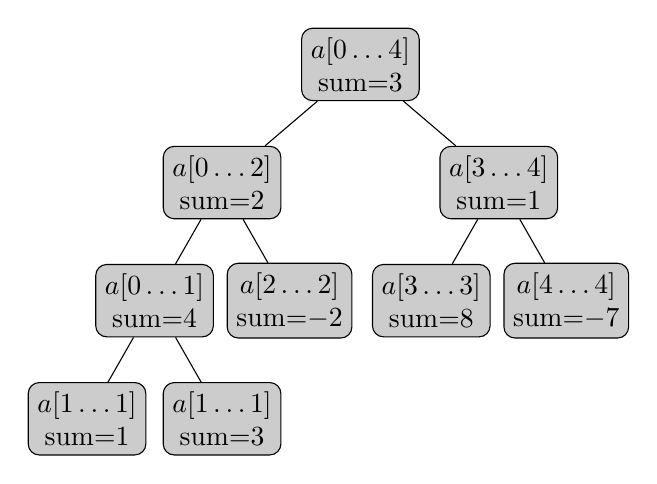
\begin{tikzpicture}[sibling distance=10em,
    every node/.style = {shape=rectangle, rounded corners,
        draw, align=center,
    fill=black!20}]]
    \node {$a[0 \dots 4]$\\sum=$3$}
        child { node {$a[0 \dots 2]$\\sum=$2$}
            child { node[xshift=9mm] {$a[0 \dots 1]$\\sum=$4$}
                child { node[xshift=9mm] {$a[1 \dots 1]$\\sum=$1$} }
                child { node[xshift=-9mm] {$a[1 \dots 1]$\\sum=$3$} }
            }
            child { node[xshift=-9mm] {$a[2 \dots 2]$\\sum=$-2$} } 
        }
        child { node {$a[3 \dots 4]$\\sum=$1$}
            child { node[xshift=9mm] {$a[3 \dots 3]$\\sum=$8$} }
            child { node[xshift=-9mm] {$a[4 \dots 4]$\\sum=$-7$} } 
        };
\end{tikzpicture}
\end{document}
